\documentclass{standalone}
\usepackage{pgfplots}
\pgfplotsset{compat=1.18} % Ensure compatibility

\begin{document}

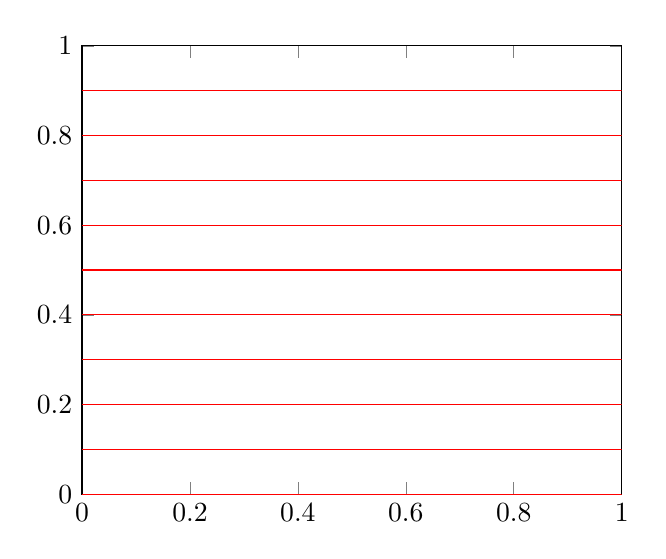
\begin{tikzpicture}
  \begin{axis}[
    ymin=0, ymax=1,
    xmin=0, xmax=1,
  ]
    \foreach \yValue in {0.00,0.1,...,1.00} {
      \edef\temp{\noexpand\draw [red] (axis cs:0,\yValue) -- (axis cs:1,\yValue);}
      \temp
    }
  \end{axis}
\end{tikzpicture}

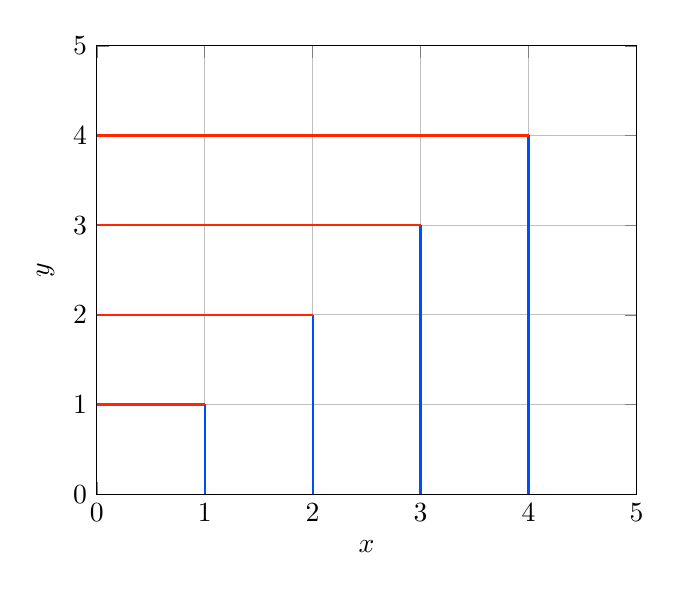
\begin{tikzpicture}
    \begin{axis}[
        xlabel=$x$,
        ylabel=$y$,
        xmin=0, xmax=5,
        ymin=0, ymax=5,
        grid=major,
    ]
        % Use \pgfplotsinvokeforeach to iterate and draw lines
        \pgfplotsinvokeforeach{1,2,3,4}{
            \addplot[thick, color=blue!70!cyan, samples=2] coordinates {(#1,0) (#1,#1)};
            \addplot[thick, color=red!70!orange, samples=2] coordinates {(0,#1) (#1,#1)};
        }
    \end{axis}
\end{tikzpicture}

\begin{tikzpicture}
\begin{axis}
\addplot[
    domain=0:10, 
    samples=100,
    thick,
    blue
] {x^2};

% Custom loop for drawing vertical lines at intervals
\foreach \i in {1, 3, ..., 9} {
    \edef\temp{\noexpand\draw[red, dashed] (\i, 0) -- (1, 1);}
        %\node[above] at (axis cs:#1, {#1^2}) {\pgfmathprintnumber{#1}};
}
\end{axis}
\end{tikzpicture}

\end{document}